

\documentclass[10pt, conference, compsocconf]{IEEEtran}

\usepackage{graphicx}
\usepackage{algorithmic,listings}
\lstset{language=C,basicstyle=\small\ttfamily, basewidth=0.51em}
\usepackage{url}
\usepackage{tabularx}
\usepackage{subfig}
\usepackage{float}
\usepackage{underscore}
\usepackage{url}
% correct bad hyphenation here
\hyphenation{op-tical net-works semi-conduc-tor}

\graphicspath{{figures/}}
\pagestyle{plain}

\newcommand\blfootnote[1]{%
  \begingroup
  \renewcommand\thefootnote{}\footnote{#1}%
  \addtocounter{footnote}{-1}%
  \endgroup
}


\begin{document}

\title{Application-Level Regression Testing Framework using Jenkins}


% author names and affiliations 
% use a multiple column layout for up to two different
% affiliations

% conference papers do not typically use \thanks and this command
% is locked out in conference mode. If really needed, such as for
% the acknowledgment of grants, issue a \IEEEoverridecommandlockouts
% after \documentclass

% for over three affiliations, or if they all won't fit within the width
% of the page, use this alternative format:
%

\author{
  \IEEEauthorblockN{Reuben D. Budiardja}
  \IEEEauthorblockA{
    National Center for Computational Sciences\\
    Oak Ridge National Laboratory, Oak Ridge, TN 37831\\
    reubendb@ornl.gov}

\and

  \IEEEauthorblockN{Timothy Bouvet, Galen Arnold}
  \IEEEauthorblockA{
    National Center for Supercomputing Applications\\
    University of Illinois at Urbana-Champaign, 61801\\
    tbouvet@illinois.edu, gwarnold@illinois.edu
  }

}

% make the title area
\maketitle
\thispagestyle{plain}

\begin{abstract}
Monitoring and testing for regression of large scale systems such as the NCSA's Blue Waters supercomputer are challenging tasks. 
In this paper we describe the solution we came up with to perform those tasks. 
Our goal was to come up with an automated solution for running user-level regression tests to evaluate system usability and performance.
Jenkins, an automation server software, was chosen for its versatility, large user base, and multitude of plugins including collecting data and plotting test results over time. 
We describe our Jenkins deployment to launch and monitor jobs on remote HPC system, perform authentication with one-time password, and integrate with our LDAP server for its authorization. 
We show some use cases and describe our best practices for successfully using Jenkins as a user-level system-wide regression testing and monitoring framework for Blue Waters.

\end{abstract}

\begin{IEEEkeywords}
System-monitoring; Regression-testing; Applications; Performance; Benchmarking
\end{IEEEkeywords}

\blfootnote{\textbf{Notice of copyright}: This manuscript has been authored by UT-Battelle, LLC under Contract No. DE-AC05-00OR22725 with the U.S. Department of Energy. The United States Government retains and the publisher, by accepting the article for publication, acknowledges that the United States Government retains a non-exclusive, paid-up, irrevocable, worldwide license to publish or reproduce the published form of this manuscript, or allow others to do so, for United States Government purposes. The Department of Energy will provide public access to these results of federally sponsored research in accordance with the DOE Public Access Plan (http://energy.gov/downloads/doe-public-access-plan).}

\section{Introduction}
\label{sec:introduction}

Monitoring large and complex high-performance computing systems has many challenges. 
Layers and multiple versions of the software stack, system-level configurations, (parallel) file systems, diversity in user needs and usage, and variable network traffic all interact to increase the system's complexity. 
Although there exist monitoring systems for each of these components, they often do not capture the behavior of the system in aggregate, which in fact is what users and their applications experience. 
Therefore an application-level system monitoring framework is needed to give us a more complete picture of the system behavior. 
 

Over time, either due to configuration and software changes or hardware aging, performance of such a complex system may regress. 
To identify and correct such regression, one must have some method to do regression testing of the system performance. 
This requires a systematic record of the system performance over time.

These two requirements can be concisely summarized as ``application-level regression testing''. 
Our goal was to implement an automated solution for running these user-level regression tests to evaluate system usability and performance. 
For this purpose we have chosen to use Jenkins \cite{jenkins}.

Jenkins is an open source automation server. 
Although it is typically used as a continuous integration tool in the software development process, its wide-ranging features makes it suitable for any task that can be automated. 
These tasks may include building applications, executing them, deploying software, and running various custom-written tests and scripts. 
We chose Jenkins as the tool for our regression testing framework because of its active development, wide community support, and the readily available ``plugins'' to perform various specific tasks.

In this paper we describe in detail our experience in using Jenkins to perform application-level regression testing on high-performance computing systems such as the Blue Water supercomputer at the National Center for Supercomputing Applications (NCSA), Darter, and Beacon at the National Institute for Computational Sciences (NICS). 
These systems are Cray XE, XK, XC, and CS series. 
The outline of this paper is as follows. In section \ref{sec:JenkinsConfiguration} we describe in detail how we configure Jenkins for our deployment. This is followed by a brief description what an application test consist of in section \ref{sec:TestAnatomy}. Section \ref{sec:UseCases} shows some use cases and results from applications we have used to monitor our systems. We end the paper with concluding remarks in section \ref{sec:Conclusion}.


\section{Jenkins Configuration}
\label{sec:JenkinsConfiguration}

\subsection{Installation}
Jenkins is typically available from the package repository of most major linux distributions. 
One can also download and install Jenkins directly from its website. 
We used the RPM package to install Jenkins on a CentOS virtual machine (VM). 
Jenkins comes with its own web server so that managing and accessing Jenkins can be done via any web browser (in the next section we discuss using Apache HTTP Server in front of Jenkin's for better security). 
Typically Jenkins's web server listens on port 8080, but this is configurable. 


\subsection{Accessing HPC Test Systems}
Jenkins has an implicit assumption that the machine on which it is installed is also the primary machine being used to build and test the software. 
In our case, this is not what we want. 
In fact, our applications will be built on the HPC system on which we intent to run the tests (typically on the login nodes), and will be run on the compute nodes of the HPC system (i.e. via batch job submission to the job queueing system). 
This is because not only do we want to test the runtime performance of the applications, but we also want to ensure that the software and programming environment of the system can build the applications correctly. 
Incidentally, the latter also informs us of any user-level problem such as slow or overloaded login nodes, slow file system access, erroneous or incompatible default software (library, compilers, etc) versions. 
In short, we want our tests to simulate the typical workflow of a user on the system being tested.

Therefore what we need is a mechanism to execute a ``project'' --- a user-configured description of work which Jenkins should perform such as building a piece of software, in Jenkins parlance --- on remote machines (``remote'' from the perspective of Jenkins). 
In this case, the Jenkins machine simply manages the automation scheduling, shows status of projects in execution (``builds'' in Jenkins parlance) , and archives results of the tests (i.e. ``artifact''). 
It also provides the user interface (via its own web server) to create and configure projects. 
These tasks are sufficiently light weight that Jenkins can be installed on a VM with sufficient disk space for the artifacts, since the truly heavy lifting on building and executing the application tests are done on the remote machine.

There are two ways to achieve an executing build on a remote machine. 
Each have their own benefits, and your selection is a matter of choice. 
One may use Jenkin's core feature of adding ``Nodes`` to its environment. 
One may also use a Jenkins plugin called ''SSH Plugin`` to allow execution on a remote machine via SSH protocol. 
At NICS our setup uses the former, while at NCSA our setup uses the latter. 
In the following we briefly discuss the setup of these two mechanisms.

\subsubsection{Using Nodes for Test Systems}
The original idea behind adding nodes is to allow Jenkins to scale with its workload. 
As projects are added, one can add nodes (i.e. more build machines) allowing Jenkins to build more projects concurrently. 
Jenkin's projects may also be explicitly 'labeled' to execute on a certain node. 
We capitalized both of these features to enable the aforementioned remote execution.

For each HPC system login node, we created a Jenkins node\footnote{Do not be confused with multiple usage of the word ''node`` here. 
The former refers to the typical usage of a login node in HPC. 
The latter refers to Jenkins' vernacular of ''node`` as previously defined}. 
We then labeled the (Jenkins) node with the name of the HPC system. 
For example, at NICS we have the labels 'beacon' and 'darter' to refer to the Cray CS-300 (Beacon) and XC-30 (Darter) login nodes, respectively. 
Each test application (i.e. ''project``) is then labeled to ensure that they only run on the appropriate node. 
For example, we have used NAMD \cite{namd} as an application test. 
We would create a Jenkins project called ''NAMD-Beacon`` and label it to run only on the ''beacon`` node. 
We would also create another project called ''NAMD-Darter`` and label it appropriately. 
The two projects have slightly different build scripts (and possibly different test cases) so that they build correctly on the systems where they were meant to run.

Jenkins nodes need to have a Java-based daemon (Jenkins' ''slave.jar``) running which connects back to the master via a certain port (which is configurable). 
This can be considered a drawback. 
If the daemon somehow dies, it needs to be restarted. 
The daemon runs as regular user, the user which essentially runs the build and submits the jobs on the HPC system. 
In our case, we created a NICS user called ''jenkins`` with the same privilege as any other regular user. 
Both the extra port opening and the daemon itself may be considered as attack vectors from a security perspective. 
At NICS however we consider this to be acceptable because of other mitigation (which we will discuss later).

The benefit of this method is that one can basically treat the nodes as a local environment in Jenkins, while having access to the HPC environment. 
For example, each node would have access to the parallel lustre filesystem mounted by the HPC system (even if Jenkins master itself does not, being only a small separate VM). 
Each node can define its lustre filesystem as its build and test workspace. 
Yet Jenkins automatically manages all communication with the nodes such that files (e.g. plot data, test output) generated on the lustre filesystem are readable from Jenkins without the explicit remote copy (i.e. via SCP). 
Another example is that one can have Jenkins checkout or clone code from a remote repository (e.g. using Subversion or Git) and the copy will be automatically available on the lustre filesystem defined as the workspace of that node. 
These integration benefits make building Jenkins projects more seamless.

\subsubsection{Using SSH Plugins for Test Systems}
The SSH plugin \cite{JenkinsSSHPlugin} is another method for which one can access the HPC systems from Jenkins. 
As the name implies, Jenkins projects with these type of build scripts simply SSH to the desired machine then execute the scripts there. 


The benefit of this method is that it more closely mimicks the way real users access the HPC system. 
There is no need for an additional daemon to run on the HPC login nodes and there is no need for the corresponding opening of a port on the Jenkins VM. 
Because NCSA and NICS systems utilize two-factor RSA one-time password for user login, one must make a slight modification so that Jenkins can have automated logins. 
The NCSA login node's \texttt{/etc/ssh/sshd_config} was modified to allow ''Public Key Authentication`` from the Jenkins VM unique IP address. 
We created an NCSA user called ''bwjenkins`` with standard user privilege. 
Pairs of SSH keys with passphrase were generated on the Jenkins VM with their public keys deployed on the appropriate login nodes in the bwjenkins user account to allow passwordless login. 
The SSH plugins allow one to manage which key (and passphrase) to use with which system. 
The keys on the Jenkins VM are located under the Jenkins home directory (by default \texttt{/var/lib/jenkins/.ssh}. 
Although this configuration can be somewhat tedious, when complete, Jenkins will be able to run scripts on the intended HPC systems via SSH. 
For testing our setup, we created simple Jenkins projects whose task is to print out the \texttt{\$HOSTNAME} of the system.

The drawback of this method is that one has to manage almost all data management explicitly. 
If one checks out or clones a repository on Jenkins (part of Jenkins core feature), it needs to be explicitly copied (e.g. with \texttt{rsync} or \texttt{scp}) to the remote system. 
Any files generated by the tests that need to be read by Jenkins (e.g. plot file) have to be copied back explicitly to the Jenkins VM. 
A related drawback is that one must explicitly ensure that the build environment is ''clean`` on the remote system (e.g. no left over files or data from previous run). 
This is because although Jenkins can clean up its workspace, this workspace (in Jenkins perspective) exists only on the VM. 
The remote systems' workspaces are out of the reach of Jenkins. 
This drawback also prevents one to easily allow concurrent builds of the same project. 



\subsection{Securing Jenkins Web Front-end}

Jenkins comes with its own web server. 
Although Jenkins also has a command-line interface, the primary way to interact with Jenkins (configuring, setting up projects, running builds) is via a web browser. 
Although the Jenkins web server may be sufficient for a setup in which Jenkins is only accessible in a secure, walled off, intranet environment, we feel that using a more secure, well-tested, production quality web server as its front end is warranted.

We decided to use an Apache HTTP Server as the front-end web server facing the world. 
To achieve that, first we set the Jenkins web server to only listen to the \texttt{localhost} interface on port 8080, by setting the following variable in Jenkins configuration file \texttt{/etc/sysconfig/jenkins}:
\begin{lstlisting}[captionpos=t,language=bash,label=lst:jenkinsConfig]
#-- Restrict to only listen to localhost
JENKINS_PORT="8080"
JENKINS_LISTEN_ADDRESS=127.0.0.1
\end{lstlisting}

Second, we need to forward all HTTP requests to Jenkins, and also forward Jenkins responses back to the client. 
This is accomplished using the module \texttt{mod_proxy} \cite{ApacheModProxy} in Apache HTTP which allows it to act as a proxy / gateway. 
To enable this feature, the following stanza is added to the configuration file \texttt{/etc/httpd/conf.d/ssl.conf} inside the \texttt{<VirtualHost>} directive:

\begin{lstlisting}[frame=b,captionpos=b,label=lst:reverseProxy,caption=Relevant configuration lines for setting up reverse proxy in Apache HTTP Server]
ProxyRequests       Off
ProxyPreserveHost   On 
AllowEncodedSlashes On 
<Proxy *>
  Order deny,allow
  Allow from all  
</Proxy>
ProxyPass   /  http://localhost:8080/ nocanon
ProxyPassReverse / http://localhost:8080/
ProxyPassReverse / http://bwjenkins.ncsa.illinois.edu/
RequestHeader set X-Forwarded-Proto "https"
RequestHeader set X-Forwarded-Port "443"    
\end{lstlisting}

With this setup, all requests to the HTTP over SSL protocol (i.e. \texttt{https}) on port 443 by default) are forwarded to the Jenkins server and Jenkins responses are forwarded back to the client (i.e. web browser).

Optionally, one may allow non-authenticated, ''read-only`` access to the Jenkins dashboard over regular (non-secure) HTTP connections. 
Jenkins' own authorization mechanism can be used to control this access, but we can also add Apache HTTP directives for further security, limiting to \texttt{GET} requests only. 
To achieve this, we created the file \texttt{/etc/httpd/conf.d/vhosts.conf} with the following content:
\begin{lstlisting}
 
NameVirtualHost *:80
<VirtualHost *:80>

  ServerAdmin tbouvet@illinois.edu
  DocumentRoot /var/www/html
  ServerName bwjenkins.ncsa.illinois.edu
  Options Indexes FollowSymLinks

  ProxyPass / http://localhost:8080/ nocanon
  ProxyPassReverse  /  http://localhost:8080/
  ProxyRequests Off
  AllowEncodedSlashes On

  LimitRequestBody 512
  LimitRequestFields 15
  LimitRequestFieldSize 1024
  LimitRequestLine 128

  <Location /asynchPeople/>
    Order Deny,Allow
    Deny from all
  </Location>

  <Proxy *>
    Order deny,allow
    Allow from all
    <LimitExcept GET>
      Deny from all
    </LimitExcept>
  </Proxy>

</VirtualHost>

\end{lstlisting}

\subsection{Authenticating with One-Time Password}

Although Jenkins supplies its own authentication mechanism with its built-in user and password database, we feel that it is inadequate for securing our instance. 
The default Jenkins authentication setup is unfortunate, in that it allows anyone to self-register creating their own username and password\footnote{This is perhaps another artifact of the Jenkins setup intended for intranet environment}. 
We wanted instead to use our One-Time Password (OTP) infrastructure with RSA SecurID \cite{RSASecurID} token for authentication. 
In this section we describe how we accomplished that.

Our use of Apache HTTP Server as front-end allow us to use ''Basic Authentication`` \cite{ApacheBasicAuth}. Via \texttt{mod_authnz_external} module \cite{ApacheModAuthExt}, one can use any external mechanism or program to authenticate. 
One example of an authenticator is the ''pwauth`` authentication program. 
It is a simple program that returns a status code given a login (username) and password. 

Combined with the Pluggable Authentication Module (PAM) --- a Unix authentication framework ---, we use ''pwauth`` to authenticate against our RSA SecurID OTP infrastructure. 
This is set up in the file \texttt{/etc/pam.d/pwauth}:
\begin{lstlisting}
#%PAM-1.0
auth	   required	/lib64/security/pam_securid.so
account    include      password-auth
\end{lstlisting}

Jenkins can use the user information given by Apache HTTP server if one selects ''HTTP Header by reverse proxy`` for its security realm. 
This means that all authentication is handled by Apache. 
Authenticating directly to \texttt{pwauth} against RSA SecurID OTP however presents an issue. 
It is often the case that a request needs to re-authenticate. 
The web browser normally handles this seamlessly by caching the user's credentials.
However, this does not work since, by definition, OTP credentials can only be used once. 
The solution is to use a back-end authenticator with some form of session management. 

To accomplish this, we wrote a small python script for managing session with OTP \cite{BasicAuthOTPSession} as the authentication mechanism, wrapping the real authenticator (i.e. \texttt{pwauth} with PAM for RSA SecurID in our case). 
When this script is initially called, it uses a pre-defined back-end authenticator for authentication. 
Once an authentication succeed, a session is created and the next request with the same credentials from the same IP address are deemed successful without going through the real authenticator. 
The session expires in a predefined amount of time. 
A new request within that time renews the session. 
If there are no more requests within that time, the session expires.
When this happens, one has to authenticate again with the back-end authenticator. 

%Figure {FIXME: CREATE FIGURE) illustrates the authentication mechanism we describe. 
Most of the configuration is defined in the file \texttt{/etc/httpd/conf.d/ssl.conf}, immediately following the stanza reproduced in listing \ref{lst:reverseProxy} inside the same \texttt{<VirtualHost>} directive:

\begin{lstlisting}
#-- OTP for Jenkins SSL connection
DefineExternalAuth pwauth+session pipe 
  /usr/local/bin/BasicAuthOTPSession.py

<LocationMatch / > 
  AuthType Basic
  AuthBasicProvider external
  AuthName "NCSA RSA OTP login" 
  AuthExternal pwauth+session
  require valid-user  
  RequestHeader unset "X-Forwarded-User"
  RequestHeader set "X-Forwarded-User" (REMOTE_USER)
</LocationMatch>
 
\end{lstlisting}
The \texttt{<LocationMatch / >} directive ensures that every request to the secure HTTP site is authenticated. 

\subsection{Authorization and Access Control}
\label{subsec:authorization}

Jenkins default authorization allows logged in (authenticated) users to have full control. 
We wanted a more fine-grained access control to our instance and therefore selected the ''matrix-based security`` option (see Figure \ref{fig:jenkinsAuthorization}). Using this option we can limit what access individual users and groups have to our Jenkins instance. 
For example we restrict most users (other than admin users) from having the ''Job Delete`` permission to prevent one user or group from deleting each other's jobs. 

\begin{figure}[h]
\centering
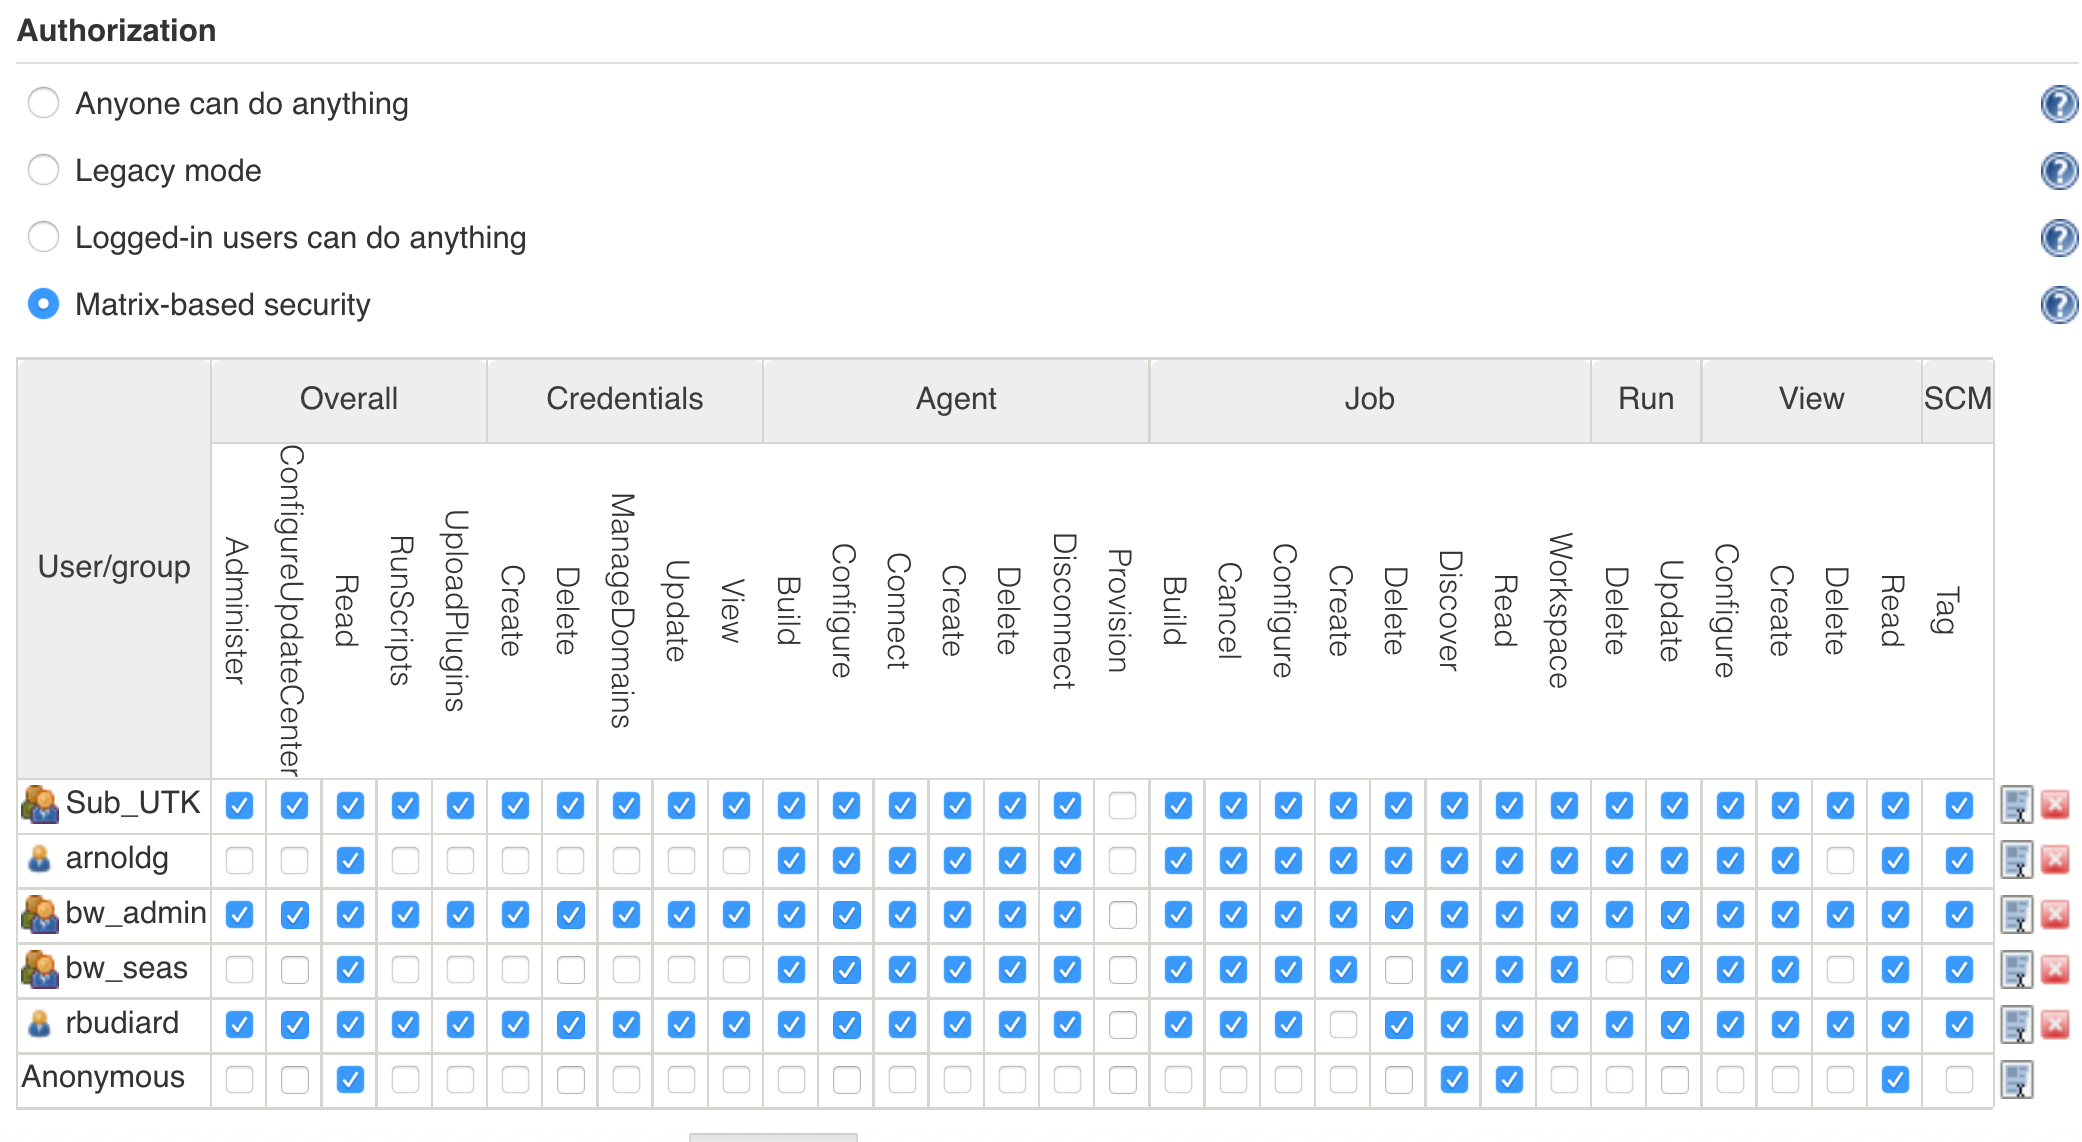
\includegraphics[width=0.5\textwidth]{Configure-Global-Security}
\caption{Jenkins fine-grained authorization.}
\label{fig:jenkinsAuthorization}
\end{figure}

We use the built-in LDAP plugin to query our LDAP server what group a user belongs to.
This greatly simplifies managing the authorization since it can be done based on groups rather than just individual users. 
The LDAP plugins gets the user information from the HTTP header passed by the reverse proxy set up. 
Figure \ref{fig:LDAP-Jenkins} shows the screenshot of our LDAP configuration within Jenkins interface.

\begin{figure}
\centering
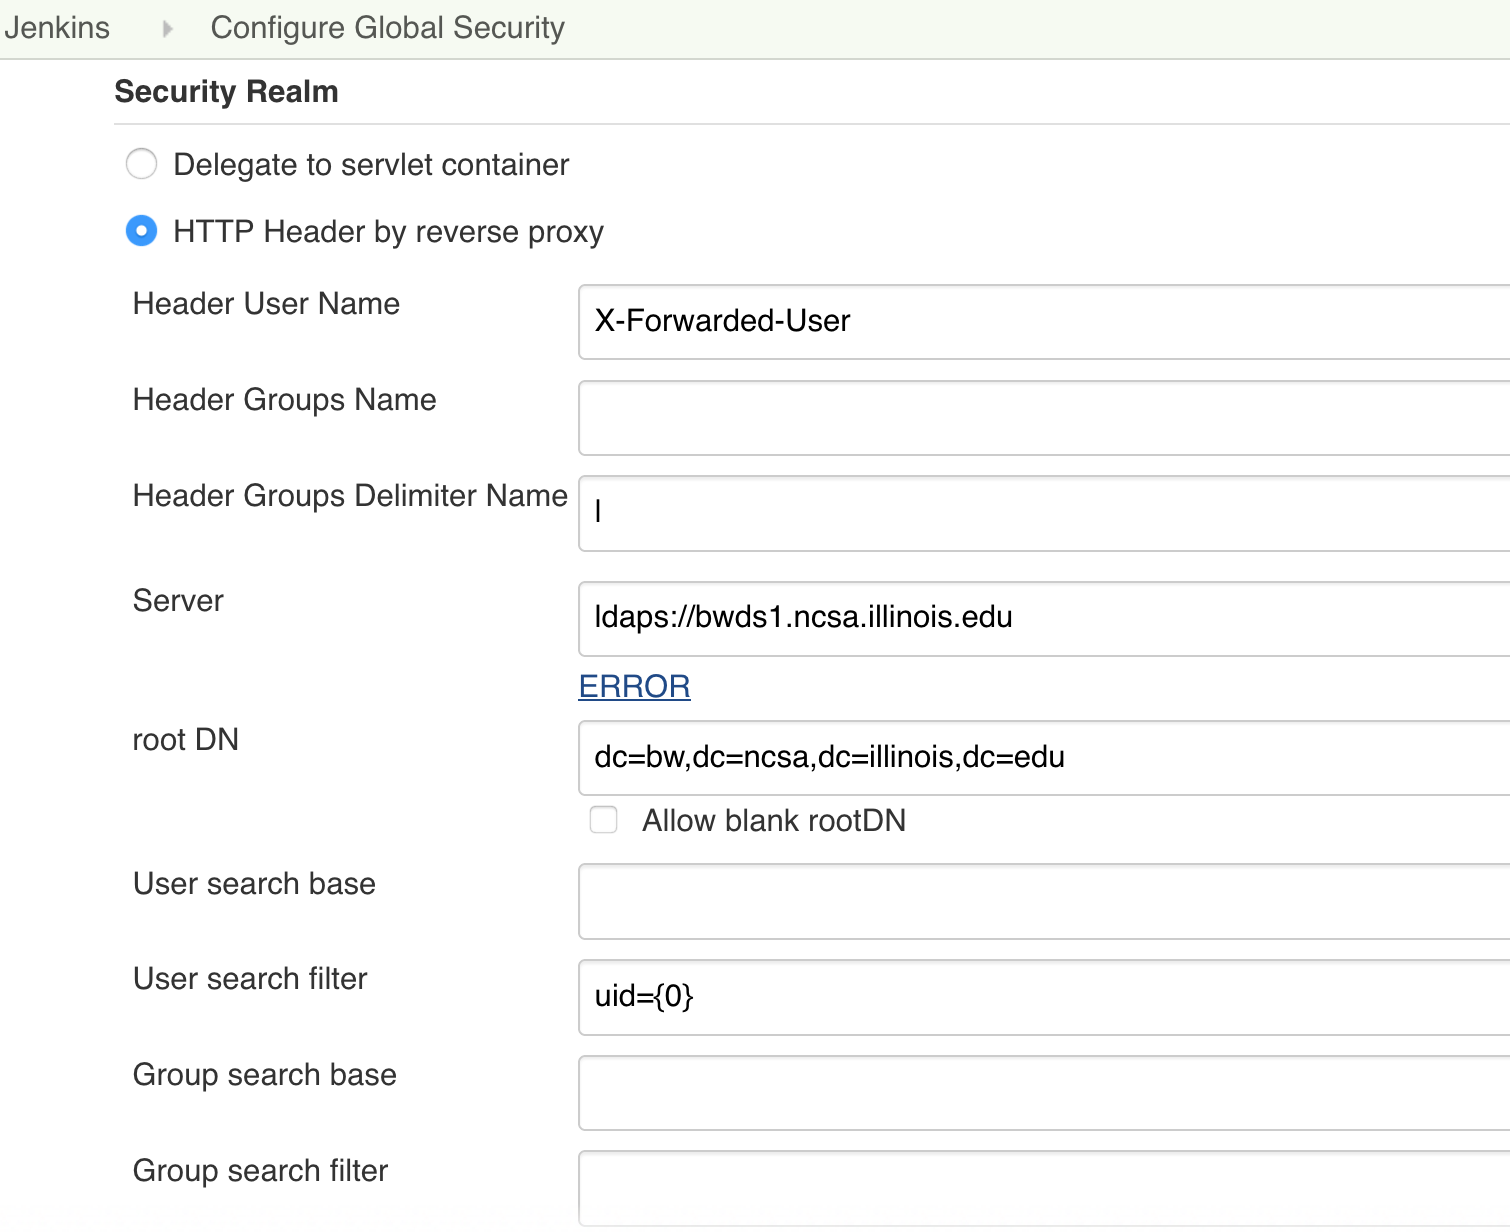
\includegraphics[width=0.5\textwidth]{LDAP-Jenkins}
\caption{Using LDAP with Jenkins.}
\label{fig:LDAP-Jenkins}
\end{figure}

Since Jenkins allows one to enter arbitrary commands to be executed on login nodes, we want to further mitigate security risk via firewall rules. 
In our installation, we only allow IP address originating from our institution block to access the secure HTTP portion and authenticate to access Jenkins. 
At NCSA, the non secure, read-only, HTTP portion is accessible from anywhere. 
At NICS, this access is only allowed from the institution IP block only. 

%/etc/sysconfig/iptables:
%-A INPUT -s 141.142.0.0/16 -m state --state NEW -m tcp 
%-p tcp --dport 22 -j ACCEPT
%-A INPUT -s 172.16.0.0/15 -m state --state NEW -m tcp 
%-p tcp --dport 22 -j ACCEPT 
%-A INPUT -m state --state NEW -m tcp -p tcp --dport 80 
%-j ACCEPT
%-A INPUT -s 141.142.0.0/16 -m state --state NEW -m tcp 
%-p tcp --dport 443 -j ACCEPT

\section{Anatomy of A Test Application}
\label{sec:TestAnatomy}
In this section we briefly describe the primary elements of a test application. 
A new test application (i.e. Jenkins job / project) must be tested on our test and development system (TDS) and approved before deployment on the user-facing production system (e.g. Blue Waters). 
\footnote{We use the terms ''test application , ''test`` (for short), ''Jenkins project``, and ''Jenkins job`` interchangeably as they refer to the same thing.}
This is one of our key best practices. 

Jenkins' dashboard by default shows the list of all Jenkins jobs under the ''All`` view tab. 
One may create different ''views`` containing a list of selected projects. 
In our case, we created several views to help us categorized our test applications.
For example, once a test application is deployed on a production environment such as Blue Waters, it is assigned to the ''BlueWaters`` view. 
This can be done by editing that view and add the selected applications to it.
Tests that are still in development reside in the "All" tab view until they have been peer reviewed by at least one other test developer.

\subsection{Name and Description}
Beyond naming the Jenkins project, we require a description for each test to describe: what is tested, the resources used by the test, the intent of the test, and the scheduling frequency of the test.

\subsection{Limiting Number of Builds Kept}
The Jenkins VM filled to capacity after the first few weeks of intensive use and an influx of several new tests that output long source code build detail.
We retroactively modified all tests to limit the number of old build logs retained (max 50 for most tests). 

\subsection{Source Code Management}
Jenkins is intended to be a continuous integration tool to assis software development, and therefore has in its core feature the ability to check out source code directly from a source code manager such as Subversion or Git (with plugin).
For our purpose, most of our tests use a specified, static version of the application and therefore do not need this functionality. 

We do have a small number of tests that automatically pulls from a repository containing SWTools2 scripts to build and test software. 
SWTools2 is a software management tools we use to install center-provided applications and libraries. Having these tests in Jenkins is useful to make sure that we can still build the software correctly with any changes in the scripts or on the systems. 
In section \ref{sec:UseCases} we show some examples of these.

\subsection{Build Triggers}
In this part we specify how the job is triggered. 
For most cases we do periodic builds with a time-based specification.

\subsection{Build Commands}
This is where we specify the (shell) commands to actually build (and run) our test application. 
This may include the actual commands to compile and link the executable, submitting jobs to the queue, and getting back and checking results.

Where possible, we try to be as transparent with our test construction as possible. 
We prefer explicit shell commands specified via Jenkins interface over running a script in the filesystem on the remote HPC system. 
Remote scripts are run with verbose mode or are displayed via \texttt{cat -n} to so that their output are captured by Jenkins console log. 
This makes it simpler for debugging when a test fails.

As described in section \ref{sec:JenkinsConfiguration}, there are two mechanisms to run these commands on the actual HPC systems. 
Using Jenkins nodes mechanism, one would select ''Execute Shell`` as the build step and put the commands there. Using the ''SSH`` mechanism, one would select ''Execute shell script on remote host using ssh``. 
The former requires that one checks the ''restrict where this project can be run`` selection to specify the HPC system. 
With the latter, in our instance there are several target ssh hosts which may be selected: the TDS (JYC), the production system (Blue Waters), and the new software deployment login node within the main system. 
None of our tests run locally within the Jenkins VM.

There are basically two kinds of tests: 

\subsubsection{Test Completes on the Login Node}
Some tests run only on the login node and return more or less immediately. 
Examples include tests for batch system functionality, login / SSH functionality, and filesystem functionality. 
These tests are very similar in style to unit tests which target a limited set of functionality.

\subsubsection{Test Submitted to Batch System}
More comprehensive tests typically build and run an application or benchmark through the batch system.  
These tests exercise multiple aspects of the system: (filesystem, compilers and modules, high-speed network, external connectivity to the internet, etc.). 
These tests are written such that they block to completion so that we do not overburden the batch system with tests. 
Unlike tests that run entirely on a login node, completion time can be highly variable depending on the queue depth and available backfill windows for the batch system.
 

Most comprehensive tests produce output that we use when debugging a failed test. 
They may also produce plot data. When using the ''SSH`` mechanism, these files are copied back to the Jenkins server so that they can be saved, viewed and/or incorporated into the plot feature of Jenkins. 
 
\subsection{Post-build Actions}

After a test is run, arbitrary numbers of post-build actions can be specified. 
The following are some that we have used. 

\subsubsection{Plots}
We installed Jenkins Plot plugin \cite{JenkinsPlotPlugin} so that successful tests can save plot files. 
The test needs to be written to generate a data point (e.g. performance value, timing, memory / IO bandwidth, etc.) to contribute to the plot. 
Under the hood, the Jenkins server accumulates the data as rows in a spreadsheet (in directory \texttt{/var/lib/jenkins/jobs/}) and plots them via the "Plots" link for a test.

\subsubsection{Email Notification}
When the state of a test changes, email notification is sent to the test owner. 
As a best practice we also use the email notification as a method of tracking authorship and each test has an email owner even if notifications are disabled for the test.

\section{Use Cases}
\label{sec:UseCases}
\subsection{IOR for Lustre Scratch Test}
We created Jenkins tests to periodically run the IOR MPI parallel I/O benchmark at modest scale and validate filesystem functionality and performance for the scratch filesystem. 
The test is scaled to provide representative performance numbers for a typical small application while not creating performance issues with other jobs or the larger filesystem.
One of our best practices is to provide a management level summary description for casual Jenkins users who want to view the tests but do not need to understand the full Jenkins configuration and execution details. 
 
\begin{figure}[H]
\centering
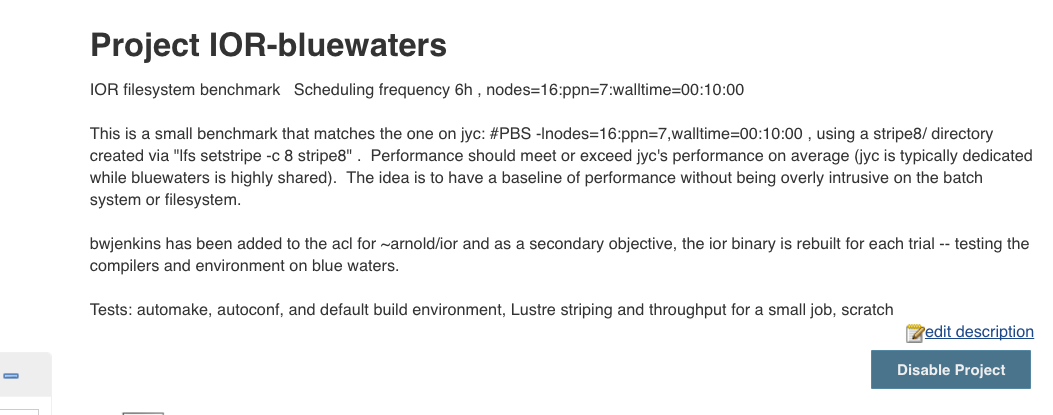
\includegraphics[width=0.5\textwidth]{IOR-bluewaters-descr}
\caption{IOR description in Jenkins.}
\label{fig:IOR-bluewaters-descr}
\end{figure}
Where possible, tests build from source and exercise multiple user-facing system components such as: Git for external connectivity and modules to test defaults in the environment. 
Where scripts on the remote SSH site are used, they are echoed and/or displayed with \texttt{cat -n} to make console output verbose and easy to debug in case of errors. 
 
\begin{figure}[H]
\centering
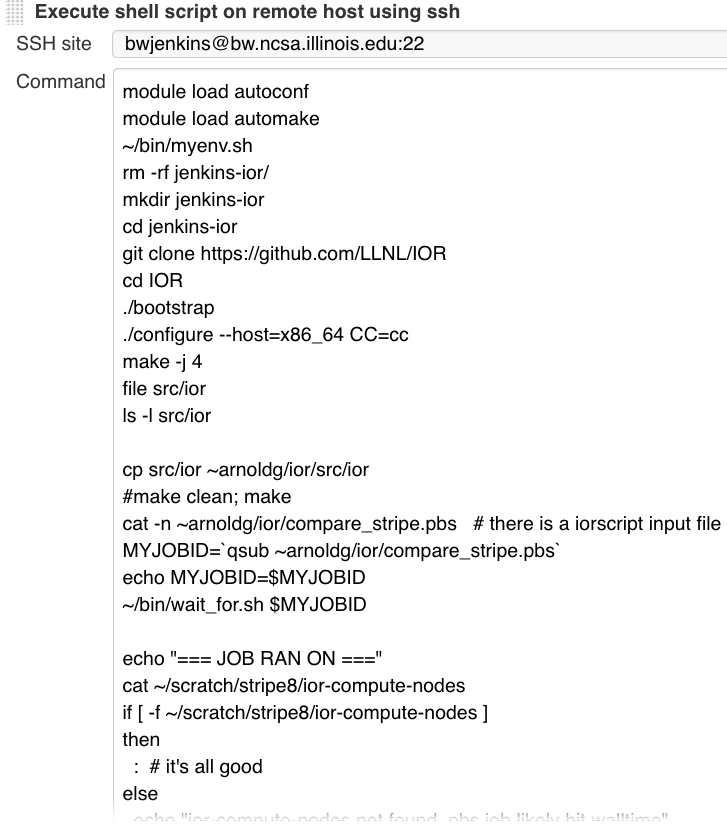
\includegraphics[width=0.5\textwidth]{IOR-configuration-sample}
\caption{ IOR configuration sample }
\label{fig:IOR-configuration-sample}
\end{figure}
The IOR test is set to run as scheduled by Jenkins with a best-effort through our batch system.
The test synchronously blocks such that the next test will not start until the previous one has completed.
We employ a watchdog script (see Listing \ref{lst:watchdog}) to monitor the batch queue and keep the test active until the system marks it as finished.
This has the side effect of making the minimum test time an integer multiple of the sleep time in the watchdog script.
This may be adjusted to fit individual site needs.
\begin{lstlisting}[frame=tb,captionpos=t,language=bash,caption={pbs/torque watchdog script}, label=lst:watchdog]
#!/bin/bash
echo "=== RUNNING $0 ==="
if [ $# -lt 1 ]
then
  echo "$0: missing argument for jobid"
  exit 1
fi
while true
do
	MYQSTAT=`qstat $1`
	if test "$MYQSTAT" = ""
        then
		echo $1 finished
		exit
	else
		DATE=`date`
		echo "$DATE: waiting for $1 to finish"
	fi
	sleep 5m
done
\end{lstlisting}

\begin{figure}[H]
\centering
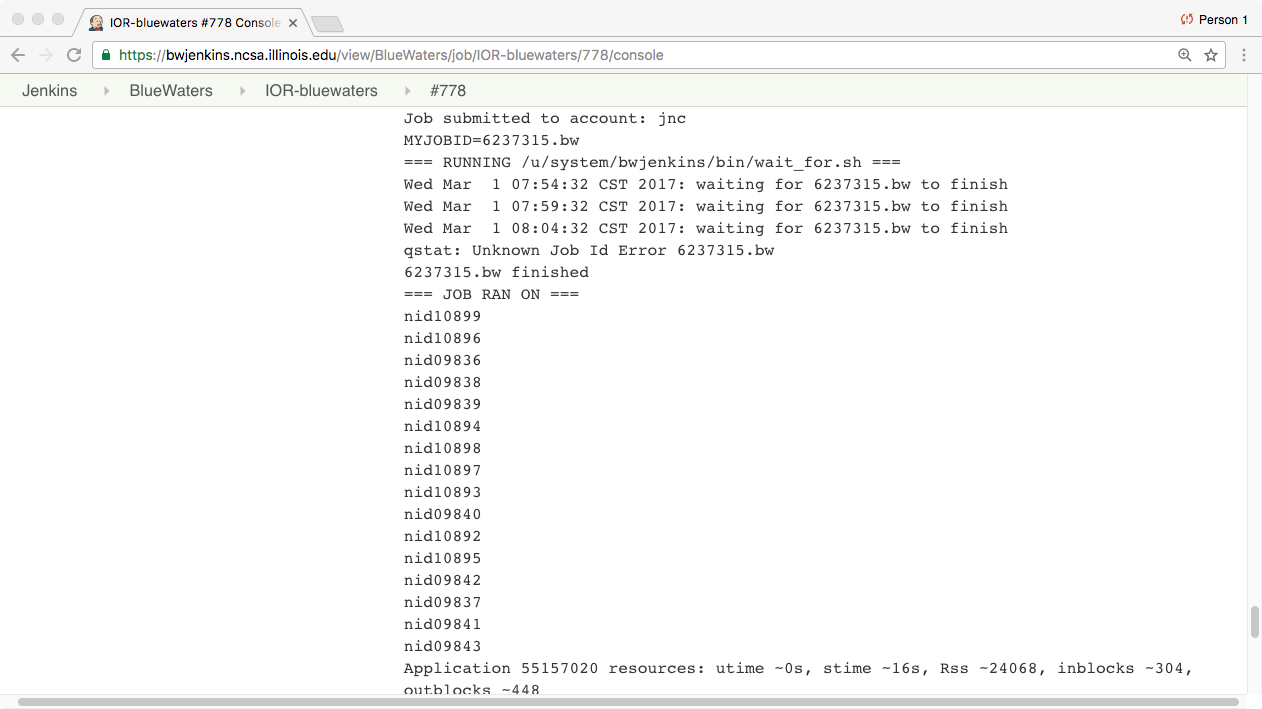
\includegraphics[width=0.5\textwidth]{IOR-watchdog-out}
\caption{ IOR watchdog console output.}
\label{fig:IOR-watchdog-out}
\end{figure}
For tests that produce an interesting performance metric like IOR, we save that output to the file format expected by Jenkins (see Listing \ref{lst:yvalue}) and use plotting feature to produce plots (Figure \ref{fig:IOR-plot}). 
\begin{lstlisting}[frame=tb,captionpos=t,language=bash,caption={sample YVALUE output file}, label=lst:yvalue]
bwjenkins$ cat myiorREADnumber.dat 
YVALUE=8352.71
\end{lstlisting}
\begin{figure}[H]
\centering
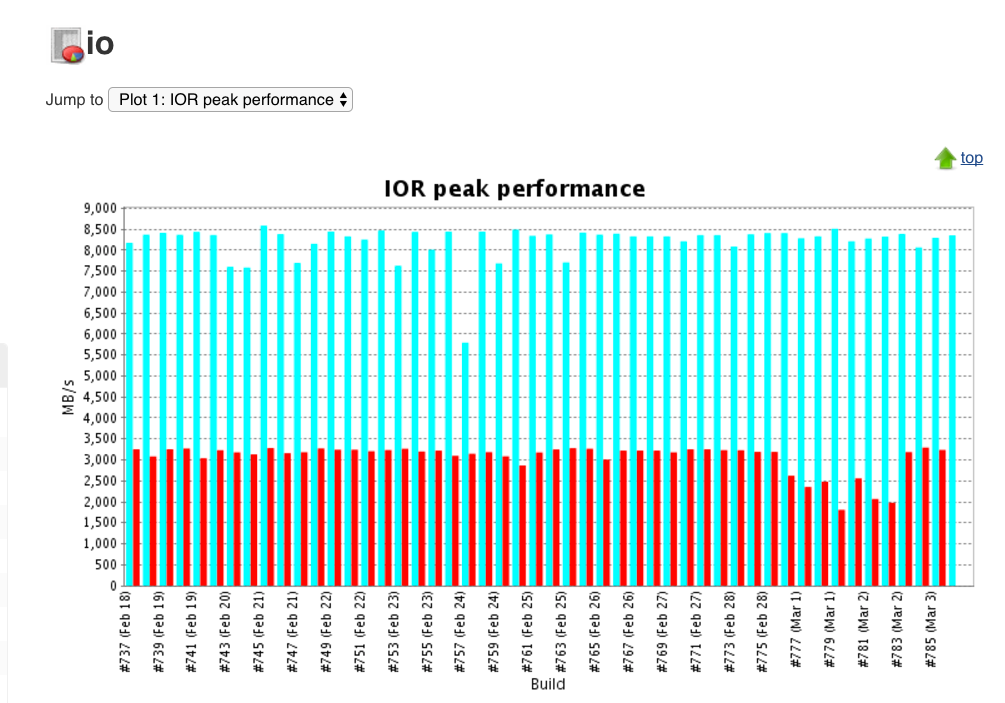
\includegraphics[width=0.5\textwidth]{IOR-plot}
\caption{IOR Plot View.}
\label{fig:IOR-plot}
\end{figure}
A plot like this helps us with performance baselines and we can quickly react to changes in the software environment or filesystem configuration that adversely impact performance.

\subsection{mdtest Lustre Tests}
The mdtest metadata test is run on the home and scratch filesystems to validate metadata server performance.  The IOR and mdtest user-facing tests complement the fine-grained detail we are able to glean from the backed system-side counters in our OVIS database where we record details about individual server metrics and network traffic on the Cray Gemini fabric. Figure \ref{fig:mdtest-plot} plots the results of this test over certain period of time. 
\begin{figure}[H]
\centering
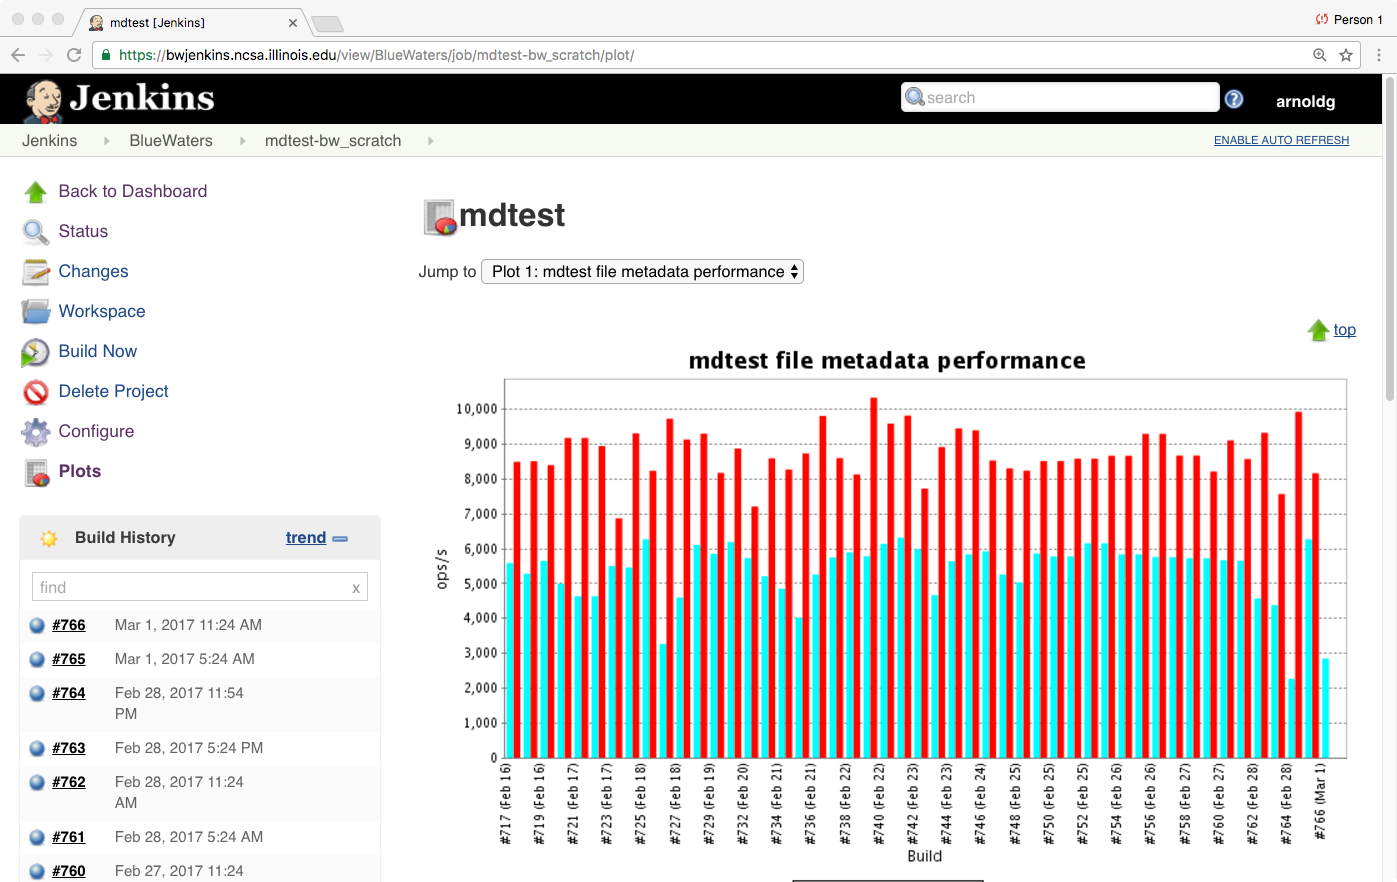
\includegraphics[width=0.5\textwidth]{mdtest-plot}
\caption{mdtest plot view }
\label{fig:mdtest-plot}
\end{figure}

An additional best practice is to enable E-mail Notifications to the test author and/or other interested parties. Setting notifications for unstable builds will trigger an e-mail every time the test state changes (from successful to failing and once again when successful ). Figure \ref{fig:mdtest-config-email} shows screenshot of the email notification configuration for the mdtest test in Jenkins.
\begin{figure}[H]
\centering
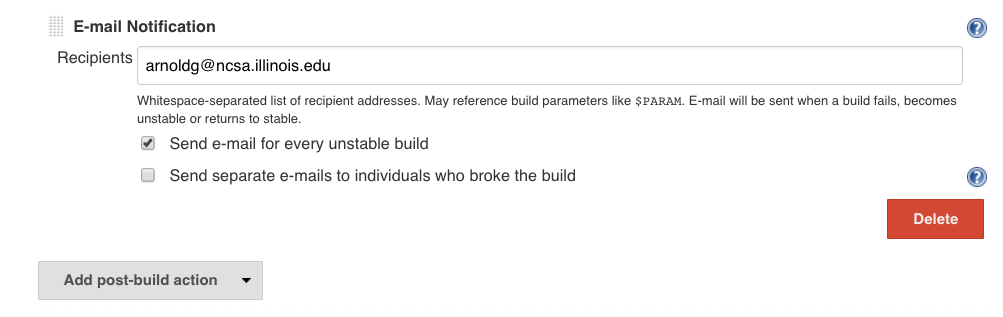
\includegraphics[width=0.5\textwidth]{mdtest-config-email}
\caption{ mdtest email configuration }
\label{fig:mdtest-config-email}
\end{figure}

\subsection{Filesystem Dashboard}
Our Jenkins instance is a source of information for a filesystem dashboard display we maintain in our wiki (Figure \ref{fig:wiki-dashboard}. The \texttt{http://} URLs for the plot images can be referred directly and are shown on the dashboard to provide a recent-time display of filesystem metrics from a user point of view. We add a Jenkins test to track response time of \texttt{/bin/ls} on the login nodes---a reasonable metric of metadata server health and also the most common problem reported by users when we are having filesystem issues.
\begin{figure}[H]
\centering
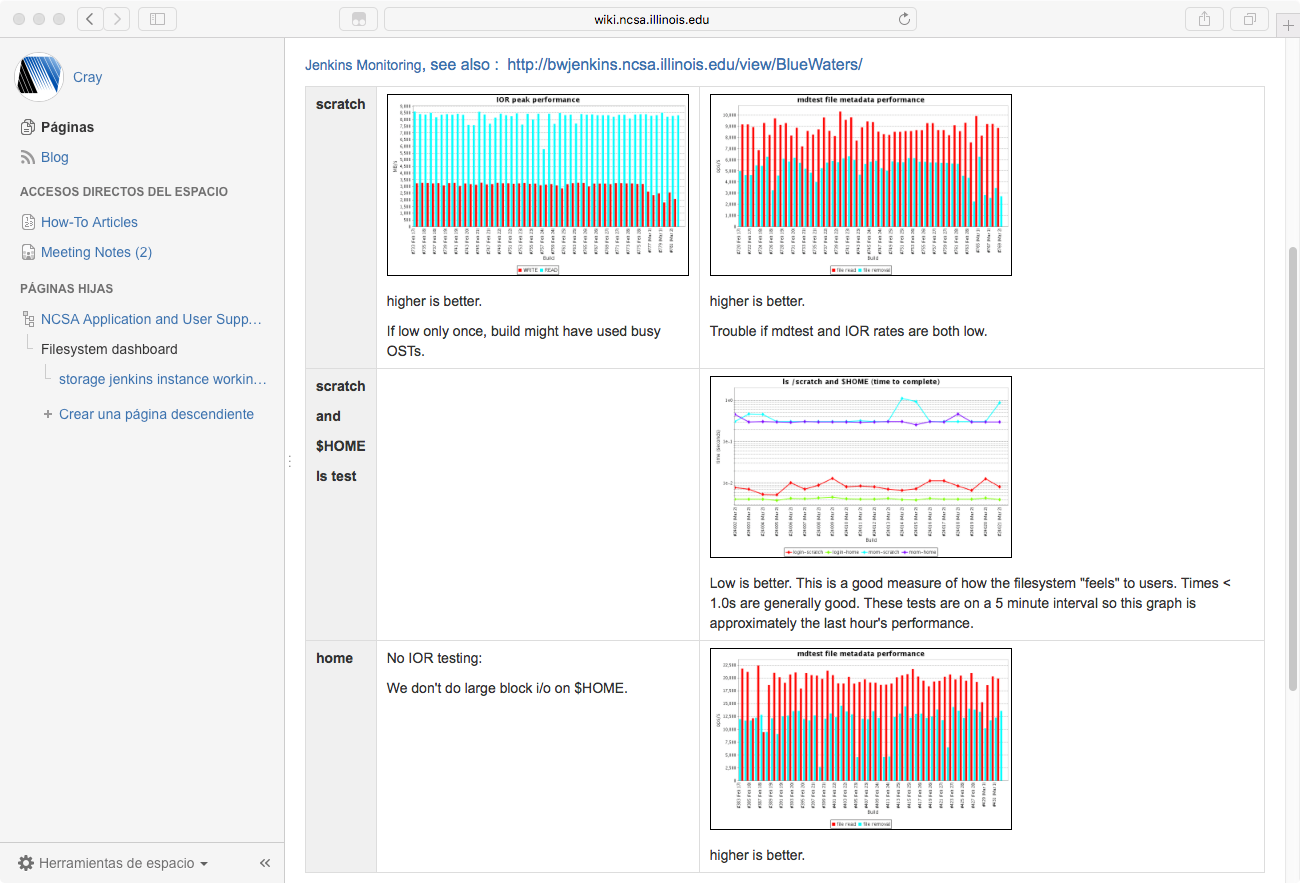
\includegraphics[width=0.5\textwidth]{wiki-dashboard}
\caption{ filesystem dashboard displaying multiple Jenkins plots }
\label{fig:wiki-dashboard}
\end{figure}

\subsection{Special Projects}
The initial display tabs (i.e. Jenkins ''Views``) in our Jenkins instance are used to group tests that are run periodically in production. We add separate ''Views`` for special projects. For example we clone existing tests for evaluating a new software stack on our test login node (''h2ologin4`` view).  Our TDS (JYC) has a separate set of tests from our production system and is used as our Jenkins development mule. The sustained petascale performance benchmarks (SPP) are in their own tab because they run at scale and are only run on-demand by staff (i.e. not scheduled to run periodically by Jenkins). Figure \ref{fig:tabs-display} illustrates our use of Jenkins views to organize our application tests.
\begin{figure}[H]
\centering
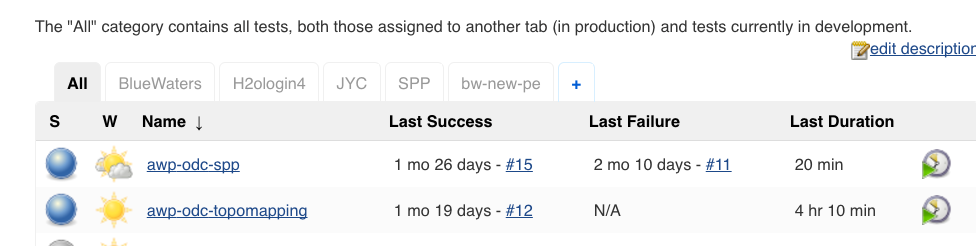
\includegraphics[width=0.5\textwidth]{tabs-display}
\caption{Jenkins views (tabs) in our instance.}
\label{fig:tabs-display}
\end{figure}

\subsection{NAMD Test}
NAMD is one of many applications provided system-wide at NICS due to its high use. It is managed via SWTools2 \cite{SWTools2} such that build and test recipes are standardized. For the purpose of regression testing, we have written several glue scripts in SWTools to make it work seamlessly in Jenkins. Figure \ref{fig:NAMD-jenkins} shows screenshot of shell commands in Jenkins interface to build and test this application. The commands hide many of the complexities of building and executing the application behind SWTools recipes for NAMD. However, they are exactly the same commands used to build and test this application for provisioning to users \footnote{SWTools recipes for this case can be gleaned at  https://github.com/reubendb/SWTools-NICS-CI}.

\begin{figure}[H]
\centering
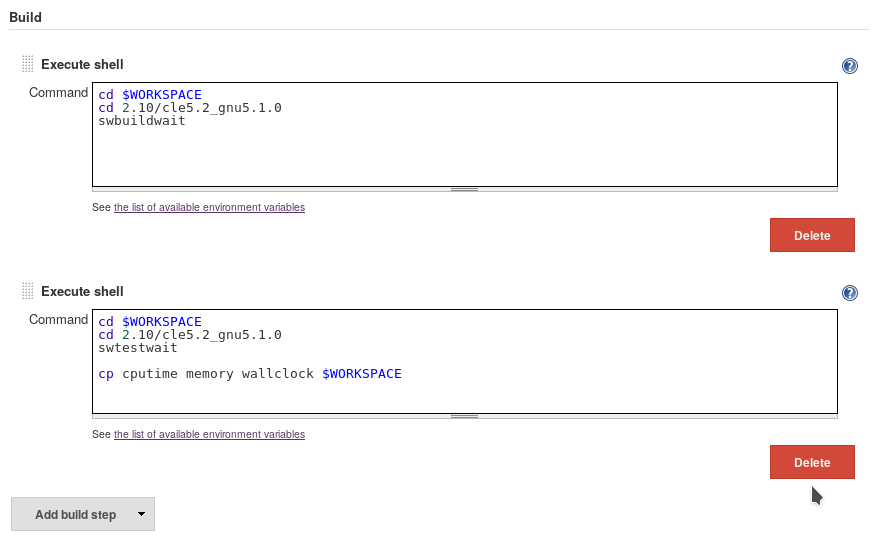
\includegraphics[width=0.5\textwidth]{NAMD-Jenkins}
\caption{Build commands for NAMD in Jenkins with SWTools2 integration.}
\label{fig:NAMD-jenkins}
\end{figure}

For this application testing, we use a well known NAMD benchmark case ''ApoA1''. We collect performance data such as CPU time and memory usage and plot them over time (see Figure \ref{fig:NAMDPlot} for screenshot of the plots as seen in Jenkins interface). 

\begin{figure}[H]
\centering
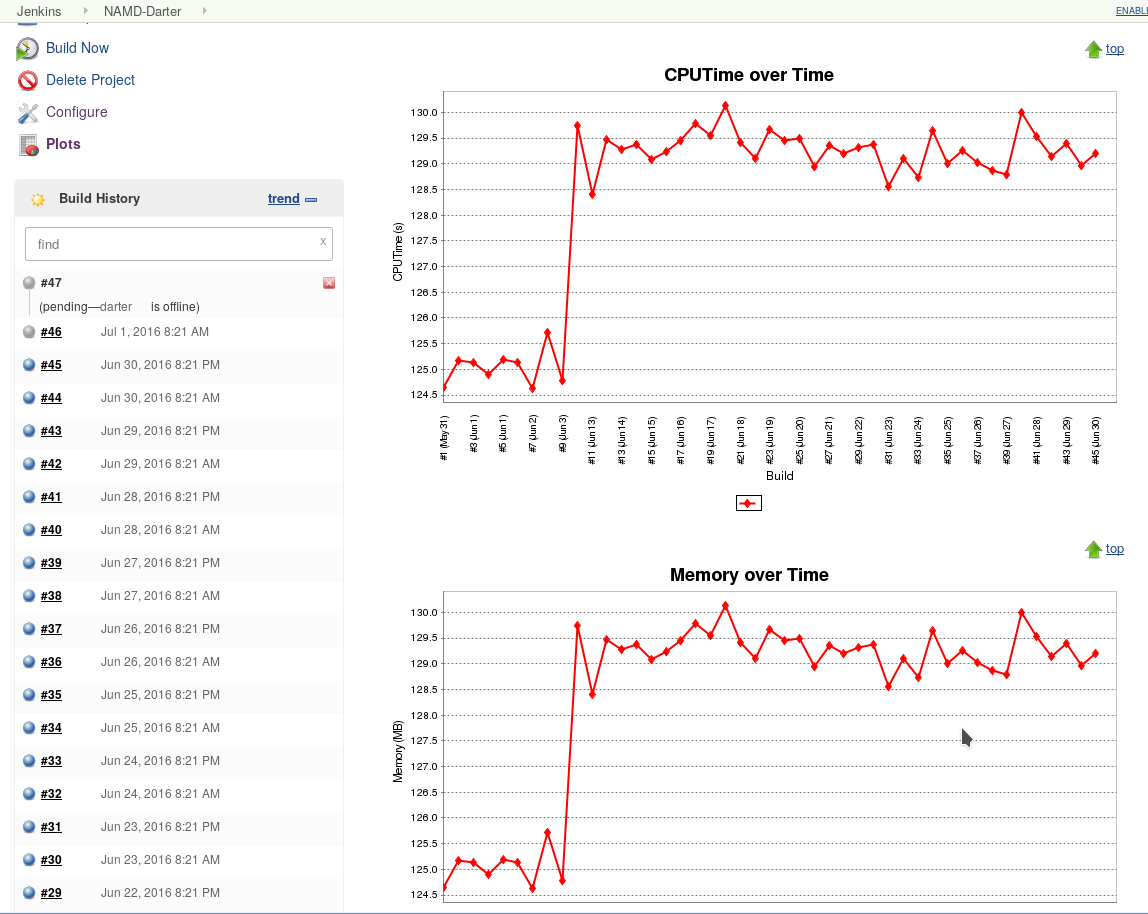
\includegraphics[width=0.5\textwidth]{NAMDPlot}
\caption{Plots of NAMD test results in Jenkins.}
\label{fig:NAMDPlot}
\end{figure}


\section{Conclusion}
\label{sec:Conclusion}

In this paper we have described our deployment of Jenkins automation server for user-level, application-based system monitoring and regression testing on large installation of HPC systems at NCSA and NICS. 
This monitoring system has proved to be useful in early detection of system issues. 

Another value of this system is to anticipate issues related to software updates. 
We typically run the latest Programming Environment (PE) on our Test and Development System (TDS), while our production systems have the latest PE installed as non default. 
During initial testing this newer PE can be loaded by modulefile selection. This setup allow us to use both the TDS and login node for testing the new software stacks and changes to the login environment without affecting the production environment. 
Jenkins projects tailored for each environment allow for regression testing of the current production as well as pre-production user-level environments with the new PE.

In developing Jenkins projects for testing, we adhere to the following best practices: 
\begin{itemize}
\item Tests are developed on the TDS and not assigned into a Jenkins tab until reviewed. 
\item Email notification is enabled for most tests and the field is always populated with a test owner.
\item All tests contain a description that describes what is tested, resources required, scheduling frequency, and overall summary  to be readable by the management team.
\item Log file count is limited in the test configuration to keep from filling filesystem space with verbose logs.
\item Tests are coded to be more verbose than necessary so that failures can be isolated quickly and easily.
\end{itemize}

In summary, our Jenkins-based system monitoring has enabled: 

\begin{itemize}
 
\item \textbf{Reproducibility and Regression Testing}: Jenkins provides the framework we need to maintain tests in a consistent fashion and track the results over time (logs and plots). 
Tests typically are not changed so that we get apples-apples comparisons.
When a new test is needed for a particular activity, we attempt to derive it from an existing test to maintain consistency and simplify test creation.
Reusable test components (watchdog scripts, plotting metrics) are employed to make construction of completely new tests straightforward.

\item \textbf{Rapid Reaction}:
The notification feature keeps test owners engaged in the testing activity of Jenkins and they are often our first responders to system issues.  This results in a shorter reaction time when the system is not performing to expectations--staff are notified automatically when the user experience is impacted.

\end{itemize}

In working with Jenkins tests, we have found that it is useful to be aware of the following caveats: 

\begin{itemize}

\item \textbf{Transient Errors}: Transient errors with Jenkins sometimes occur--particularly with the Jenkins ssh subsystem. 
It's not unusual to get ssh failure rates of 1/100 which are completely transient (immediately running the test again manually clears the issue on the dashboard).

\item \textbf{Test Scale and Frequency}: There is some subjectivity in the frequency and scale (resource utilization) of tests.
Testing too often, too large, or some combination of the two may perturb the system such that other tests are impacted or create bottlenecks in the system for the real user community.
This is the primary reason we require peer review for new tests.
\end{itemize}

Due to our initial successful deployment of Jenkins as regression testing framework on NCSA and NICS resources,  it is currently being deployed on other resources including the CADES (Compute and Data Environment for Science) resources at the Oak Ridge National Laboratory. 

% use section* for acknowledgement
\section*{Acknowledgment}
We thank Gary Rogers at NICS for his help in setting up and testing OTP integration. This research used resources at the National Institute for Computational Sciences (NICS) and the National Center for Supercomputing Applications (NCSA), funded by the National Science Foundation (NSF).  

% References
\bibliographystyle{unsrt}
\bibliography{references}


\end{document}
